% \iffalse
\let\negmedspace\undefined
\let\negthickspace\undefined
\documentclass[journal,12pt,twocolumn]{IEEEtran}
\usepackage{cite}
\usepackage{amsmath,amssymb,amsfonts,amsthm}
\usepackage{algorithmic}
\usepackage{graphicx}
\usepackage{textcomp}
\usepackage{xcolor}
\usepackage{txfonts}
\usepackage{listings}
\usepackage{enumitem}
\usepackage{mathtools}
\usepackage{gensymb}
\usepackage{comment}
\usepackage[breaklinks=true]{hyperref}
\usepackage{tkz-euclide} 
\usepackage{listings}
\usepackage{gvv}                                        
\def\inputGnumericTable{}                                 
\usepackage[latin1]{inputenc}                                
\usepackage{color}                                            
\usepackage{array}                                            
\usepackage{longtable}                                       
\usepackage{calc}                                             
\usepackage{multirow}                                         
\usepackage{hhline}                                           
\usepackage{ifthen}                                           
\usepackage{lscape}
\usepackage[center]{caption} % center the captions to figure

\newtheorem{theorem}{Theorem}[section]
\newtheorem{problem}{Problem}
\newtheorem{proposition}{Proposition}[section]
\newtheorem{lemma}{Lemma}[section]
\newtheorem{corollary}[theorem]{Corollary}
\newtheorem{example}{Example}[section]
\newtheorem{definition}[problem]{Definition}
\newcommand{\BEQA}{\begin{eqnarray}}
\newcommand{\EEQA}{\end{eqnarray}}
\newcommand{\define}{\stackrel{\triangle}{=}}
\theoremstyle{remark}
\newtheorem{rem}{Remark}
\begin{document}

\newcolumntype{M}[1]{>{\centering\arraybackslash}m{#1}}
\newcolumntype{N}{@{}m{0pt}@{}}

\bibliographystyle{IEEEtran}
\vspace{3cm}

\title{NCERT 11.9.5} % TODO: change wrong problem number
\author{ee23btech11223 - Soham Prabhakar More% <-this % stops a space
}
\maketitle
\newpage
\bigskip

\renewcommand{\thefigure}{\theenumi}
\renewcommand{\thetable}{\theenumi}

\bibliographystyle{IEEEtran}

\textbf{Question:}\\
Which term of the following sequences:\\
(a) 2,$2\sqrt{2}$,4\dots is 128
\quad(b) $\sqrt{3}$,3,$3\sqrt{3}$\dots is 729\\
(c) $\frac{1}{3}$,$\frac{1}{9}$,$\frac{1}{27}$\dots is $\frac{1}{19683}$

\textbf{Answer:} (a) Let $x_1\brak{0} = 2$, $r_1 = \frac{2\sqrt{2}}{2} = \sqrt{2}$, then the general term is:
\begin{align}
    x_1\brak{n} = x_1\brak{0} r_1^nu[n]
\end{align}
where u[0] = 1. Assume $n^{th}\brak{n > 0}$ term is 128: 
\begin{align}
    x_1\brak{n} &= x_1\brak{0} r^n = 128\\
    \implies r_1^{n} &= \frac{128}{x_1\brak{0}}\\
    \implies n &= \log_{r_1}{\frac{128}{x_1\brak{0}}}
\end{align}
Using values from \tabref{Table:1}, 
\begin{align}
    \implies n &= \log_{\sqrt{2}}{\frac{128}{2}}\\
    \implies n &= \log_{\sqrt{2}}{64}\\
    \implies n &= \log_{\sqrt{2}}{\sqrt{2}^{12}}\\
    \therefore n &= 12
\end{align}
Thus the $13^{th}$ term of the G.P $x_1\brak{n}$ is 128.\\ 
\begin{figure}[h!]
    \centering
    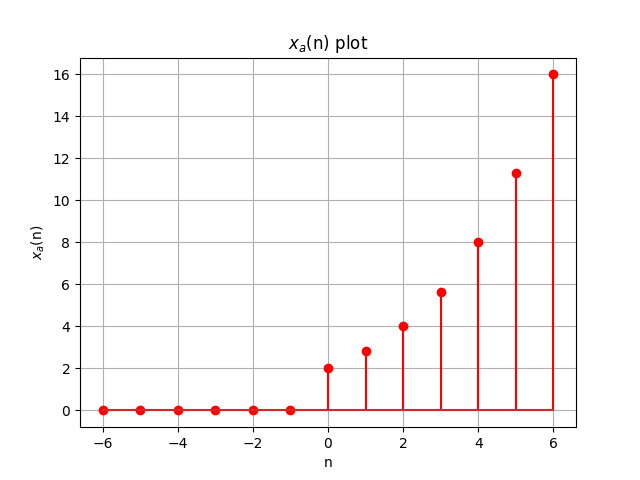
\includegraphics[width=0.5\textwidth]{figs/a.png}
    Fig. 1: Plot of $x_1$\brak{n} from n = -6 to 6
    \label{fig:img1}
\end{figure}


Let $x\brak{n} = x\brak{0}r^nu[n]$ be a general sequence then it's Z-transform:
\begin{align}
    X\brak{z} &= \sum_{n = -\infty}^{\infty}{x\brak{n} \cdot z^{-n}}\\
    \implies X\brak{z} &= \sum_{n = 0}^{\infty}{x\brak{0}r^{n}z^{-n}}\\
    \implies X\brak{z} &= x\brak{0}\sum_{n = 0}^{\infty}{r^n z^{-n}}\\
    \implies X\brak{z} &= \frac{x\brak{0}}{r}(\frac{1}{1 - \frac{r}{z}})\\
    \therefore X\brak{z} &= \frac{x\brak{0}z}{r(z - r)} \forall {\abs{z} > \abs{r}} \label{zresult}
\end{align}
\begin{align}
    \therefore X_1\brak{z} = \frac{\sqrt{2}z}{z - \sqrt{2}}
\end{align}
with ROC: \[ \abs{z} > \sqrt{2} \]

(b) Let $x_2\brak{0} = \sqrt{3}$, $r_2 = \frac{3}{\sqrt{3}} = \sqrt{3}$, then the general term is:
\begin{align}
    x_2\brak{n} = x_2\brak{0} r_2^nu[n]
\end{align}
where u[0] = 1. Assume $n^{th}\brak{n > 0}$ term is 729, which gives: 
\begin{align}
    x_2\brak{n} &= x_2\brak{0} r_2^n = 729\\
    \implies r_2^n &= \frac{729}{x_2\brak{0}}\\
    \implies n &= \log_{r_2}{\frac{729}{x_2\brak{0}}}
\end{align}
Using values from \tabref{Table:1},
\begin{align}
    \implies n &= \log_{\sqrt{3}}{\frac{729}{\sqrt{3}}}\\
    \implies n &= \log_{\sqrt{3}}{\frac{3^6}{\sqrt{3}}}\\
    \implies n &= \log_{\sqrt{3}}{\sqrt{3}^{11}}\\
    \therefore n &= 11
\end{align}
Thus the $12^{th}$ term of the G.P $x_2\brak{n}$ is 729. \\

By eqn \ref{zresult}, the Z-transform of $x_2$\brak{n}:
\begin{align} X_2\brak{z} = \frac{z}{z - \sqrt{3}} \end{align}
with ROC: \[ \abs{z} > \sqrt{3} \]

\begin{figure}[h!]
    \centering
    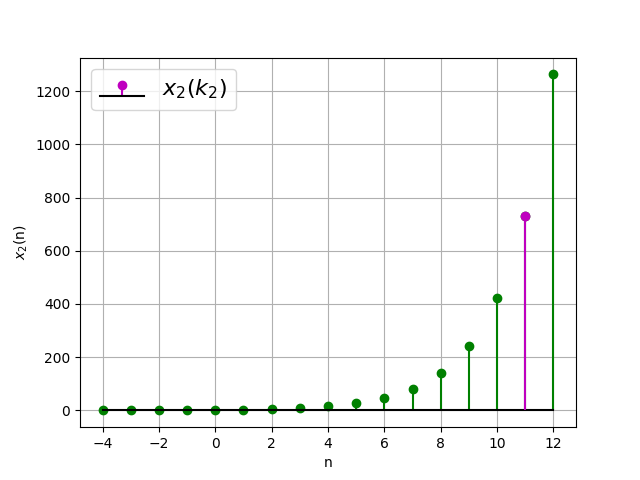
\includegraphics[width=0.5\textwidth]{figs/b.png}
    Fig. 2: Plot of $x_2$\brak{n} from n = -6 to 6
    \label{fig:img2}
\end{figure}

(c) Let $x_3\brak{0} = \frac{1}{3}$, $r_3 = \frac{\frac{1}{9}}{\frac{1}{3}} = \frac{1}{3}$, then the general term is:
\begin{align}
    x_3\brak{n} = x_3\brak{0} r_3^nu[n]
\end{align}
where u[0] = 1. Assume $n^{th}\brak{n > 0}$ term is $\frac{1}{19683}$, which gives: 
\begin{align}
    x_3\brak{n} &= x_3\brak{0} r_3^n = \frac{1}{19683}\\
    \implies r_3^n &= \frac{1}{19683 x_3\brak{0}}\\
    \implies n &= \log_{r_3}{\frac{1}{19683 x_3\brak{0}}}
\end{align}
Using values from \tabref{Table:1},
\begin{align}
    \implies n &= \log_{\frac{1}{3}}{\frac{1}{19683 \frac{1}{3}}}\\
    \implies n &= \log_{\frac{1}{3}}{\frac{1}{6561}}\\
    \implies n &= \log_{\frac{1}{3}}{3^{-8}}\\
    \therefore n &= 8
\end{align}
Thus the $9^{th}$ term of the G.P $x_3\brak{n}$ is $\frac{1}{19683}$.\\
By eqn \ref{zresult}, the Z-transform of $x_3\brak{n}$:
\begin{align}
    X_3\brak{z} = \frac{z}{z - \frac{1}{3}}
    \implies X_3\brak{z} = \frac{3z}{3z - 1}
\end{align} with ROC: \[ \abs{z} > \frac{1}{3} \]

\begin{figure}[h!]
    \centering
    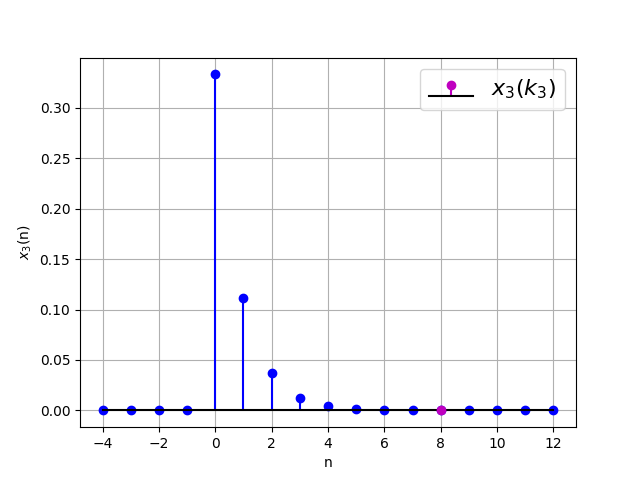
\includegraphics[width=0.5\textwidth]{figs/c.png}
    Fig. 3: Plot of $x_3$\brak{n} from n = -6 to 6
    \label{fig:img3}
\end{figure}

\renewcommand\thetable{1}
\begin{tabular}{|c|c|}
    \hline 
    \textbf{Parameter}&\textbf{Description} \\
    \hline
    $F\brak{s}$ & Laplace transform of $\delta\brak{t - a}$ \\
    \hline
    $G\brak{f}$ & Fourier transform of $\delta\brak{t - a}$ \\
    \hline
    $w_T\brak{t}$ & Delta Comb, $\sum_{k = -\infty}^{\infty}\delta\brak{t - kT}$ \\
    \hline
    $W_T\brak{t}$ & Fourier transform of $w_T\brak{t}$ \\
    \hline
\end{tabular}

\caption{Table of parameters}
\label{Table:2022.ME.3.1}



\end{document}

